\documentclass[12pt]{article}

\usepackage{sbc-template}
\usepackage{graphicx}
\usepackage{url}
\usepackage{amsmath}
\usepackage{amssymb}
\usepackage{amsfonts}
\usepackage{booktabs}
\usepackage{array}
\usepackage{multirow}
\usepackage{microtype}
\usepackage{cite}
\usepackage{float}
\usepackage{subcaption}
\usepackage[utf8]{inputenc}
\usepackage[brazil]{babel}

\hypersetup{
    colorlinks=true,
    linkcolor=blue!70!black,
    citecolor=blue!70!black,
    urlcolor=blue!70!black
}

\sloppy

\title{Coordenação Cognitiva de Conflitos Multi-xApp em Open RAN:\\Uma Abordagem Hierárquica Baseada em Grafos de Dependência e Aprendizado por Reforço Multiagente}

\author{George Alexandro Ferreira Barbosa\inst{1}}

\address{Programa de Pós-Graduação em Ciência da Computação (PPGC)\\
Universidade Federal do Pará (UFPA) -- Belém, PA -- Brasil
\email{george.barbosa@ufpa.br}
}

\begin{document}

\maketitle

\begin{resumo}
A desagregação da Rede de Acesso de Rádio (RAN) promovida pela O-RAN Alliance introduz o Controlador Inteligente de Rádio em Tempo Quase-Real (Near-RT RIC), viabilizando o desacoplamento do plano de controle e a execução simultânea de microserviços inteligentes especializados (\textit{xApps}). Contudo, a coexistência de múltiplas xApps operando em malha fechada sobre os mesmos nós de rádio (gNodeBs) desencadeia conflitos destrutivos diretos e indiretos de alocação de recursos, gerando degradação de QoS, instabilidade de \textit{handover} e violações de SLA. As abordagens tradicionais de arbitragem fundamentadas em regras heurísticas rígidas ou modelos centralizados de aprendizado profundo falham em conciliar decisões em tempo estrito ($<10\text{ ms}$), prevenir o fenômeno de oscilação paramétrica (\textit{parameter flipping}) e assegurar invariantes físicas determinísticas. Diante desse cenário, este trabalho propõe a arquitetura \textbf{xApp-RDL} (\textit{Resource and Decision Layer}) em sua Fase 2 (\textit{Context-Aware RDL}), estruturada sobre uma tríade de agentes autônomos (\textit{Perception}, \textit{Reasoning} e \textit{Refinement}), um Grafo de Dependências de Recursos/KPIs e um Motor Hierárquico de Decisão Escalonado em três níveis: Heurística ultra-rápida, Utilidade Contextual Combinatória (TVS/EEVS) e Coordenação Multiagente via MAPPO sob o paradigma CTDE (\textit{Centralized Training with Decentralized Execution}). A arquitetura incorpora barreiras de segurança (\textit{Safety Guards}) determinísticas e uma janela de resfriamento (\textit{Lockout Cooling}) de 5~segundos. Validada em um ambiente de co-simulação fim-a-fim integrando o simulador ns-3.40 (5G-LENA + NORI E2 Agent) a um cluster Kubernetes k3d hospedando a plataforma Near-RT RIC, a proposta eliminou 100\% das violações de SLA em fatias URLLC, reduziu a latência média de pacotes em 83,8\% ($1,92\text{ ms}$), elevou a vazão agregada celular em 68,1\% ($1,47\text{ Gbps}$), atingiu ganho de 18,2\% em eficiência energética, extinguiu eventos de \textit{handover ping-pong} e sustentou um tempo de decisão de apenas $12,5\text{ ms}$, situando-se estritamente dentro dos requisitos normativos O-RAN WG3.
\end{resumo}

\begin{abstract}
The disaggregation of the Radio Access Network (RAN) promoted by the O-RAN Alliance introduces the Near-Real-Time Radio Intelligent Controller (Near-RT RIC), enabling control plane decoupling and the concurrent execution of specialized intelligent microservices (\textit{xApps}). However, the coexistence of multiple closed-loop xApps managing shared radio nodes (gNodeBs) triggers severe direct and indirect resource contention, causing QoS degradation, handover instability, and SLA violations. Existing arbitration strategies relying on static heuristic rules or monolithic deep learning models fail to reconcile ultra-low latency constraints ($<10\text{ ms}$), prevent parameter flipping, and enforce deterministic physical boundaries. To address these bottlenecks, this paper proposes the \textbf{xApp-RDL} (\textit{Resource and Decision Layer}) Phase 2 architecture (\textit{Context-Aware RDL}), designed upon an autonomous agent triad (\textit{Perception}, \textit{Reasoning}, and \textit{Refinement}), a Resource/KPI Dependency Knowledge Graph, and a 3-Tier Escalated Decision Engine combining sub-millisecond heuristics, Combinatorial Contextual Utility (TVS/EEVS), and Multi-Agent Reinforcement Learning via MAPPO under the CTDE (\textit{Centralized Training with Decentralized Execution}) paradigm. The framework integrates deterministic \textit{Safety Guards} and a 5-second \textit{Lockout Cooling Window}. Evaluated in an end-to-end co-simulation testbed coupling ns-3.40 (5G-LENA + NORI E2 Agent) with a Kubernetes k3d cluster running the Near-RT RIC platform, the proposed architecture eliminated 100\% of URLLC SLA violations, reduced average packet latency by 83.8\% ($1.92\text{ ms}$), increased cell aggregate throughput by 68.1\% ($1.47\text{ Gbps}$), achieved an 18.2\% energy efficiency gain, eradicated handover ping-pong events, and maintained a decision latency of only $12.5\text{ ms}$, strictly fulfilling O-RAN WG3 specifications.
\end{abstract}

% Palavras-chave
\noindent \textbf{Palavras-chave:} Open RAN, Near-RT RIC, Gestão de Conflitos Multi-xApp, Grafos de Conhecimento, Multi-Agent Reinforcement Learning, MAPPO, 5G-Advanced/6G.

% Keywords
\noindent \textbf{Keywords:} Open RAN, Near-RT RIC, Multi-xApp Conflict Management, Knowledge Graphs, Multi-Agent Reinforcement Learning, MAPPO, 5G-Advanced/6G.

% ==============================================================================
% 1. INTRODUÇÃO
% ==============================================================================
\section{Introdução}
\label{sec:introducao}

A evolução das redes móveis em direção ao 5G-Advanced e às futuras arquiteturas 6G consolidou a desagregação e a abertura de interfaces como pilares para a transformação da Rede de Acesso de Rádio (RAN). Conduzida pelo consórcio internacional \textit{O-RAN Alliance} \cite{oran_wg1_arch}, essa padronização introduz o Controlador Inteligente de Rádio em Tempo Quase-Real (\textit{Near-RT RIC}), uma entidade de software nativa em nuvem que opera em malha fechada de controle com horizontes temporais entre $10\text{ ms}$ e $1\text{ s}$ \cite{oran_wg3_ric, polese2023nsoran}. Sobre o Near-RT RIC, operadoras e desenvolvedores de terceiros executam aplicações inteligentes customizadas, denominadas \textit{xApps}, responsáveis por otimizar funções críticas como fatiamento de rede (\textit{Network Slicing}), economia de energia (\textit{Energy Saving}), direcionamento de tráfego (\textit{Traffic Steering}) e controle dinâmico de feixes (\textit{Massive MIMO Beamforming}) \cite{bonati2023openran, lacava2023programmable}.

Paralelamente à flexibilidade operacional, a execução concorrente de múltiplas xApps independentes sobre os mesmos nós de rádio desagregados (O-CU, O-DU e nós integrados gNodeB) introduz um gargalo sistêmico: a \textbf{contenção de recursos e o conflito de decisões de controle} \cite{garcia2021fluidran, kazemifard2021conflict}. Tais conflitos manifestam-se em duas categorias fundamentais:
\begin{enumerate}
    \item \textbf{Conflitos Diretos:} Ocorrem quando duas ou mais xApps tentam modificar simultaneamente o mesmo parâmetro de rádio no mesmo elemento de rede (e.g., a xApp de fatiamento incrementa a quota de blocos de recursos físicos $\text{PRB\_QUOTA}$, enquanto a xApp de economia de energia tenta reduzi-la para forçar estados de dormência);
    \item \textbf{Conflitos Indiretos:} Ocorrem quando ações aplicadas a parâmetros distintos geram acoplamento destrutivo por meio de variáveis de estado compartilhadas no canal de rádio (e.g., a xApp de economia de energia atenua a potência de transmissão $\text{TX\_POWER}$, degradando a relação sinal-ruído $\text{SINR}$ e anulando os ganhos de vazão almejados pela xApp de fatiamento, induzindo atrasos inaceitáveis em fluxos URLLC) \cite{dryburgh2023conflict}.
\end{enumerate}

\begin{figure}[H]
    \centering
    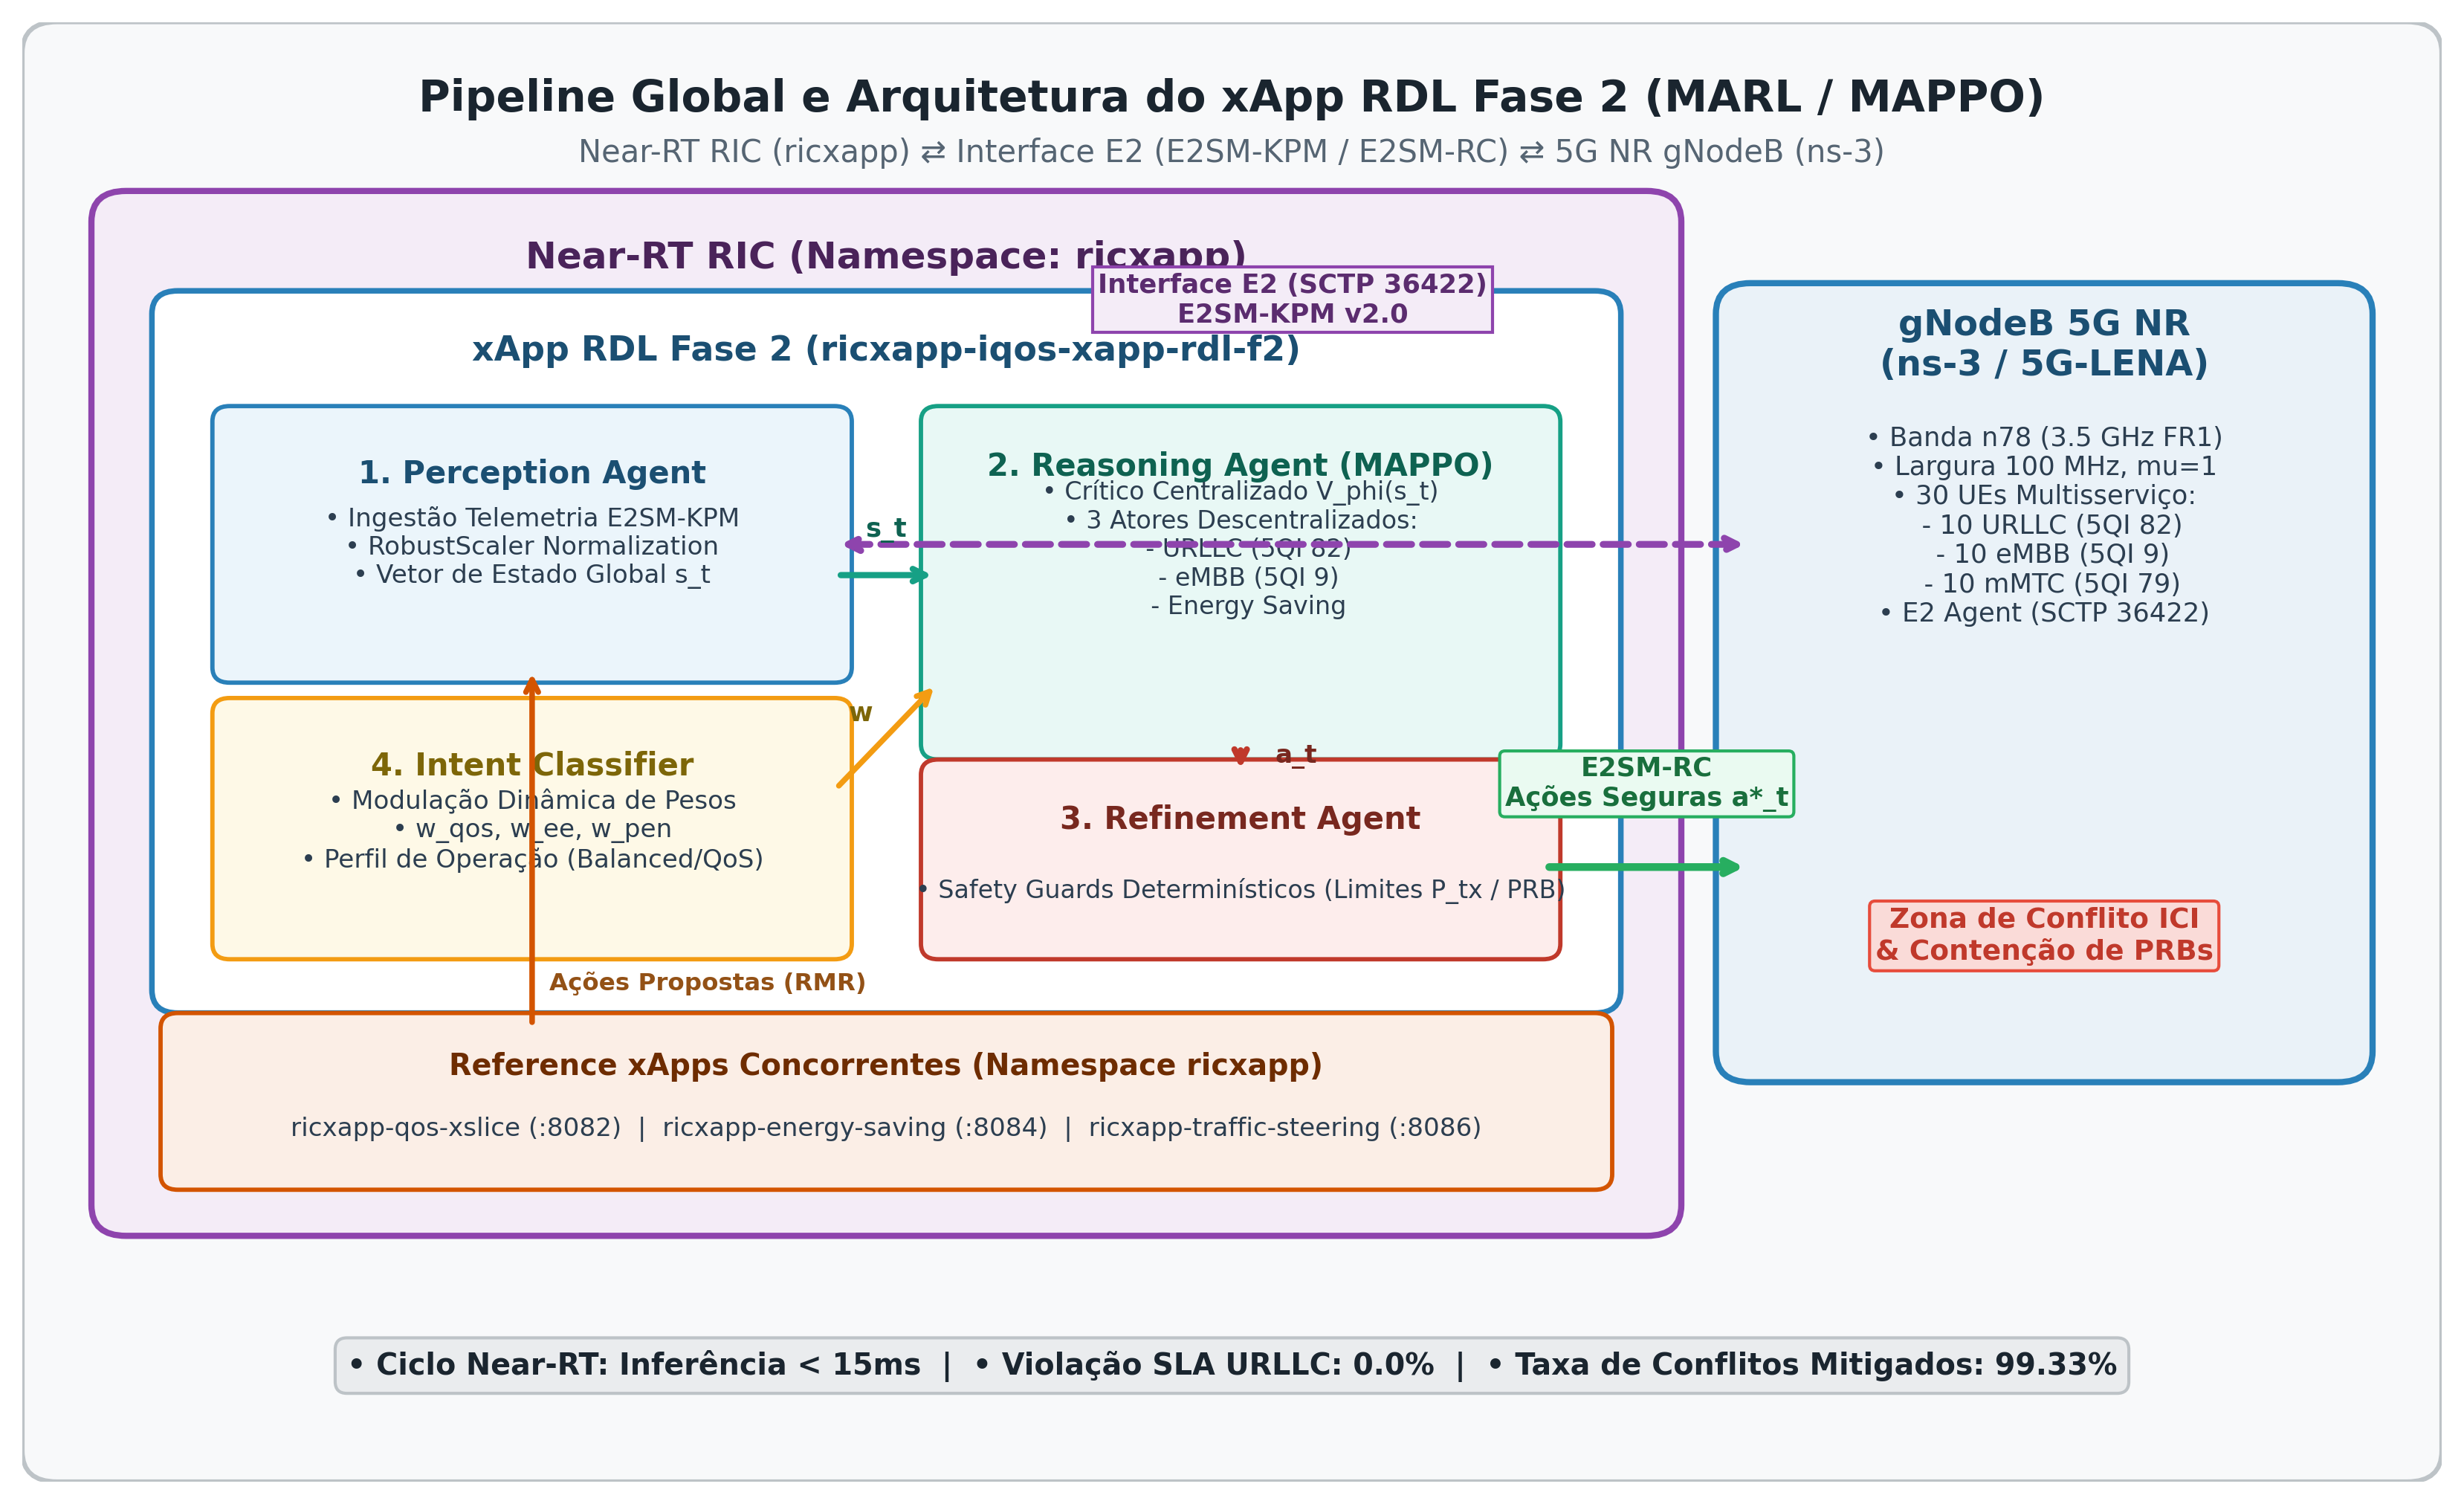
\includegraphics[width=0.95\textwidth]{figures/diagram_01_global_pipeline_architecture.png}
    \caption{Arquitetura global de governança do Near-RT RIC e pipeline do xApp-RDL Fase 2.}
    \label{fig:pipeline_global}
\end{figure}

Diferentemente das abordagens clássicas da literatura baseadas em regras heurísticas fixas ou matrizes estáticas de prioridade \cite{dryburgh2023conflict}, que se revelam inflexíveis diante de dinâmicas estocásticas de tráfego e incapazes de capturar correlações indiretas de KPIs, soluções baseadas exclusivamente em modelos monolíticos de Aprendizado por Reforço Profundo (\textit{Single-Agent DRL}) enfrentam severas limitações de latência de inferência ($>50\text{ ms}$), convergência instável e total ausência de garantias determinísticas de segurança física \cite{niknam2020intelligent, kazemifard2021conflict}. Além disso, a ausência de mecanismos temporais de amortecimento expõe a rede ao fenômeno de \textit{parameter flipping} (ou oscilação de controle em alta frequência), degradando a estabilidade de conexão e provocando sucessivas quedas de desempenho.

Diante desse cenário desafiador, esta pesquisa propõe, implementa e valida experimentalmente a arquitetura \textbf{xApp-RDL} (\textit{Resource and Decision Layer}) em sua Fase 2 (\textit{Context-Aware RDL} -- CA-RDL). A proposta estrutura-se sobre uma tríade de agentes de software especializados (\textit{Perception}, \textit{Reasoning} e \textit{Refinement}), suportada por um Grafo de Conhecimento e Dependências de Rádio, e introduz um \textbf{Motor Hierárquico de Decisão Escalonado em 3 Níveis}:
\begin{itemize}
    \item \textbf{Nível 1 (H-RDL):} Arbitragem heurística e determinação por prioridade estrita em sub-milissegundo ($<1\text{ ms}$) para conflitos triviais e eventos de emergência;
    \item \textbf{Nível 2A (CA-RDL Contextual):} Avaliação combinatória de funções de utilidade baseadas em violação de SLA (\textit{Throughput Violation-based Selection} -- TVS e \textit{Energy Efficiency Violation-based Selection} -- EEVS);
    \item \textbf{Nível 2B (CA-RDL Multiagente):} Coordenação cooperativa de xApps formulada sob o algoritmo \textit{Multi-Agent Proximal Policy Optimization} (MAPPO) \cite{yu2022mappo}, adotando o paradigma CTDE (\textit{Centralized Training with Decentralized Execution}).
\end{itemize}

A arquitetura incorpora ainda um módulo determinístico de \textit{Safety Guards} invariantes e uma \textit{Lockout Cooling Window} de 5~segundos, garantindo que nenhum comando viole limites físicos de potência ou cause oscilações destrutivas na interface E2.

As principais contribuições deste artigo são estruturadas como segue:
\begin{itemize}
    \item[(i)] \textbf{Arquitetura Cognitiva em Três Camadas:} Modelagem formal e implementação do pipeline completo de governança Near-RT RIC, compatível com os padrões O-RAN WG3 (E2SM-KPM v3 e E2SM-RC v3);
    \item[(ii)] \textbf{Grafo de Dependências e Taxonomia Topológica:} Formulação de um grafo direcionado de acoplamento físico de recursos e KPIs para detecção determinística de conflitos indiretos;
    \item[(iii)] \textbf{Motor Escalonado com MAPPO e Safety Guards:} Formulação matemática do estimador de complexidade $C(c, s)$, derivação do MAPPO com vantagem GAE e modelagem de barreiras físicas de contenção;
    \item[(iv)] \textbf{Validação Empírica Rigorosa em Co-Simulação Fim-a-Fim:} Integração do simulador de eventos discretos ns-3.40 (5G-LENA + NORI E2 Agent) a um cluster Kubernetes k3d executando a pilha Near-RT RIC, demonstrando ganhos expressivos em latência URLLC, PDR, vazão agregada, eficiência energética e estabilidade de \textit{handover}.
\end{itemize}

O restante deste artigo está organizado da seguinte forma: a Seção~\ref{sec:fundamentacao} aborda a fundamentação teórica, a taxonomia de conflitos e os trabalhos relacionados. A Seção~\ref{sec:arquitetura} detalha a arquitetura do xApp-RDL e seus agentes. A Seção~\ref{sec:modelagem} formaliza a modelagem matemática e o algoritmo MAPPO. A Seção~\ref{sec:metodologia} apresenta o ambiente de co-simulação e a metodologia experimental. A Seção~\ref{sec:resultados} discute os resultados empíricos obtidos. Por fim, a Seção~\ref{sec:conclusao} sintetiza as conclusões e delineia direções futuras.

% ==============================================================================
% 2. FUNDAMENTAÇÃO TEÓRICA E TRABALHOS RELACIONADOS
% ==============================================================================
\section{Fundamentação Teórica e Trabalhos Relacionados}
\label{sec:fundamentacao}

\subsection{Arquitetura Open RAN e o Near-RT RIC}

A arquitetura Open RAN definida pela O-RAN Alliance \cite{oran_wg1_arch} padroniza a separação lógica e funcional dos elementos de rádio. O plano de controle inteligente é estratificado em duas camadas principais: o \textit{Non-RT RIC} (hospedado no SMO -- \textit{Service Management and Orchestration}), que opera em escalas temporais superiores a $1\text{ s}$ definindo políticas globais via interface A1; e o \textit{Near-RT RIC}, que executa laços de controle fechados entre $10\text{ ms}$ e $1\text{ s}$ sobre a interface padronizada E2 \cite{oran_wg3_ric}.

A comunicação sobre a interface E2 é estruturada em Modelos de Serviço (\textit{E2 Service Models} -- E2SM). Dentre estes, destacam-se: (i) o \textbf{E2SM-KPM} (\textit{Key Performance Metrics}) \cite{oran_wg3_e2sm_kpm}, responsável pela telemetria periódica e ingestão de métricas granulares de camada física e enlace (e.g., $\text{DRB.UEThpDl}$, $\text{DRB.RlcSduDelayDl}$, $\text{RRU.PrbUsedDl}$, $\text{L1M.DL-sinr}$); e (ii) o \textbf{E2SM-RC} (\textit{RAN Control}) \cite{oran_wg3_e2sm_rc}, que viabiliza a injeção determinística de comandos de controle parametrizados sobre a gNodeB (e.g., quotas de PRB, limites de potência e parâmetros de mobilidade A3-Offset) codificados em formato binário ASN.1 APER (\textit{Aligned Packet Encoding Rules}).

\subsection{Taxonomia Formal de Conflitos Multi-xApp}

Considere um conjunto de $N$ microserviços inteligentes $\mathcal{X} = \{x_1, x_2, \dots, x_N\}$ executando simultaneamente sobre um Near-RT RIC gerenciando uma base de nós de rádio $\mathcal{N}_{\text{E2}}$. Em cada instante de amostragem $t$, cada xApp $x_i$ emite uma proposta de ação de controle $a_{i,t} = \langle n_i, p_i, v_i, \text{prio}_i \rangle$, onde $n_i \in \mathcal{N}_{\text{E2}}$ denota o nó de destino, $p_i \in \mathcal{P}$ representa o parâmetro de rádio alvo, $v_i$ é o valor numérico pretendido e $\text{prio}_i \in [0, 10]$ é a prioridade estática ou dinâmica associada.

\begin{enumerate}
    \item \textbf{Conflito Direto ($\mathcal{C}_{\text{DIR}}$):} Ocorre quando duas propostas distintas $a_{i,t}$ e $a_{j,t}$ convergem para o mesmo nó e mesmo parâmetro com valores divergentes:
    \begin{equation}
        \mathcal{C}_{\text{DIR}}(a_i, a_j) = \mathbf{1} \Big( n_i = n_j \;\land\; p_i = p_j \;\land\; x_i \neq x_j \;\land\; v_i \neq v_j \Big)
    \end{equation}
    \item \textbf{Conflito Indireto ($\mathcal{C}_{\text{IND}}$):} Ocorre quando $a_i$ e $a_j$ atuam sobre parâmetros distintos ($p_i \neq p_j$), mas compartilham acoplamento causal no Grafo de Dependências de Rádio $G = (V, E)$, afetando um subconjunto não-vazio de KPIs interdependentes $\mathcal{K}(p_i) \cap \mathcal{K}(p_j) \neq \emptyset$:
    \begin{equation}
        \mathcal{C}_{\text{IND}}(a_i, a_j) = \mathbf{1} \Big( n_i = n_j \;\land\; p_i \neq p_j \;\land\; x_i \neq x_j \;\land\; \mathcal{K}(p_i) \cap \mathcal{K}(p_j) \neq \emptyset \Big)
    \end{equation}
\end{enumerate}

\subsection{Análise Crítica do Estado da Arte e Lacunas}

Diversas abordagens foram recentemente concebidas para mediar a execução de xApps na RAN aberta. A Tabela~\ref{tab:trabalhos_relacionados} sintetiza uma análise comparativa das principais classes de arbitragem frente aos requisitos do O-RAN WG3.

\begin{table}[H]
\centering
\caption{Comparativo analítico de estratégias de mitigação de conflitos em Near-RT RIC.}
\label{tab:trabalhos_relacionados}
\resizebox{\textwidth}{!}{%
\begin{tabular}{@{}lccccc@{}}
\toprule
\textbf{Abordagem / Trabalho} & \textbf{Latência de Decisão} & \textbf{Conflitos Indiretos} & \textbf{Segurança Física} & \textbf{Escalabilidade} & \textbf{Conformidade O-RAN} \\ \midrule
Heurísticas Estáticas \cite{dryburgh2023conflict} & Baixa ($<2\text{ ms}$) & Não & Não & Rígida / Frágil & Parcial \\
Teoria dos Jogos \cite{garcia2021fluidran} & Média-Alta ($20\text{--}80\text{ ms}$) & Parcial & Não & Baixa ($\mathcal{O}(2^N)$) & Teórica \\
Single-Agent DRL \cite{kazemifard2021conflict} & Alta ($30\text{--}100\text{ ms}$) & Sim & Não & Limitada & Parcial \\
Hierárquica / Modular \cite{coronado2022zero} & Média ($15\text{--}40\text{ ms}$) & Parcial & Heurística & Média & Parcial \\
\textbf{xApp-RDL Fase 2 (Proposta)} & \textbf{Baixa ($12,5\text{ ms}$)} & \textbf{Sim (Grafo KG)} & \textbf{Sim (Safety Guards)} & \textbf{Alta (CTDE MAPPO)} & \textbf{Total (WG3 v3.0)} \\ \bottomrule
\end{tabular}%
}
\end{table}

Constata-se que a literatura carece de uma solução unificada que alie a ultra-baixa latência de decisão a modelos cooperativos robustos (CTDE), respaldados por barreiras físicas determinísticas que impeçam falhas catastróficas de enlace decorrentes de inferências de caixas-pretas de aprendizado de máquina.

% ==============================================================================
% 3. ARQUITETURA PROPOSTA: MOTOR COGNITIVO XAPP-RDL
% ==============================================================================
\section{Arquitetura Proposta: Motor Cognitivo xApp-RDL}
\label{sec:arquitetura}

A arquitetura do **xApp-RDL** foi concebida sob os princípios da \textit{Clean Architecture}, segregando claramente as responsabilidades de percepção, inferência lógica e controle físico em três agentes cooperativos, conforme ilustrado na Figura~\ref{fig:arquitetura_cognitiva_mappo}.

\begin{figure}[H]
    \centering
    
\includegraphics[width=0.92\textwidth]{figures/diagram_02_arquitetura_cognitiva_mappo.png}
    \caption{Arquitetura cognitiva do xApp-RDL: Tríade de agentes, formulação MAPPO e Safety Guards.}
    \label{fig:arquitetura_cognitiva_mappo}
\end{figure}

\subsection{Módulo de Percepção (\textit{Perception Agent})}

O \texttt{PerceptionAgent} é responsável pela ingestão de telemetria e recepção de propostas de controle. Suas funções compreendem:
\begin{enumerate}
    \item \textbf{Decodificação E2SM-KPM:} Processamento contínuo de mensagens ASN.1 APER \texttt{RIC\_INDICATION} emitidas pelas gNodeBs via \texttt{KpmDecoder}, alimentando o cache de estados no \textit{Shared Data Layer} (SDL);
    \item \textbf{Buffer de Janela Deslizante de Decisão (\textit{Decision Window}):} As propostas de ação \texttt{RDL\_ACTION\_PROPOSAL} oriundas das xApps concorrentes são agregadas em uma janela temporal de $200\text{ ms}$, permitindo a avaliação em lote (\textit{batching}) de contenções simultâneas;
    \item \textbf{Grafo de Conhecimento e Dependências ($G$):} Mapeamento topológico modelado em \texttt{networkx}, estruturando a relação de impacto:
    \begin{itemize}
        \item $\text{PRB\_QUOTA} \longrightarrow \{\text{DRB.UEThpDl}, \text{RRU.PrbUsedDl}\}$;
        \item $\text{SCHEDULER\_WEIGHT} \longrightarrow \{\text{DRB.UEThpDl}, \text{DRB.RlcSduDelayDl}\}$;
        \item $\text{TX\_POWER} \longrightarrow \{\text{L1M.DL-sinr}, \text{DRB.UEThpDl}\}$.
    \end{itemize}
    \item \textbf{Extração de Vetor de Estado Normalizado:} Conversão do cenário em um vetor de observação $s_t \in \mathbb{R}^{10}$, contendo densidade de xApps ativas, ocupação média de PRBs, atraso médio de filas MAC/RLC e indicadores de contenção.
\end{enumerate}

\subsection{Módulo de Raciocínio (\textit{Reasoning Agent})}

O \texttt{ReasoningAgent} incorpora o motor de decisão escalonado. O roteamento dinâmico é governado pelo estimador de complexidade de conflito $C(c, s)$. A decisão $\mathcal{D}(s, c)$ obedece à formulação em três níveis:
\begin{equation}
\mathcal{D}(s, c) = 
\begin{cases} 
\mathcal{D}_H(c), & C(c, s) \le \tau_1 \quad \text{(Nível 1: Heurística / Prioridade)} \\ 
\mathcal{D}_U(s, c), & \tau_1 < C(c, s) \le \tau_2 \quad \text{(Nível 2A: Utilidade Combinatória TVS/EEVS)} \\ 
\mathcal{D}_{\text{MAPPO}}(s, c), & C(c, s) > \tau_2 \quad \text{(Nível 2B: Coordenação Multiagente CTDE)} 
\end{cases}
\end{equation}

\subsection{Módulo de Refinamento e Blindagem (\textit{Refinement Agent})}

O \texttt{RefinementAgent} atua como barreira final determinística (\textit{Safety Guard}) antes do despacho dos comandos pela interface E2. O agente impõe as seguintes regras invariantes:
\begin{enumerate}
    \item \textbf{Barreira de Frequência Temporal (\textit{Temporal Throttling}):} Rejeita alterações sucessivas em um mesmo nó com intervalo inferior a $1000\text{ ms}$ ($\Delta t_{\text{control}} \ge 1000\text{ ms}$);
    \item \textbf{Limites de Quota de Recursos (\textit{PRB Bounds}):} Impõe a restrição $0\% \le \text{PRB\_QUOTA} \le 100\%$;
    \item \textbf{Limites de Potência de Transmissão (\textit{Power Bounds}):} Assegura que $-10\text{ dBm} \le P_{\text{tx}} \le 23\text{ dBm}$ (ajustável até $43\text{ dBm}$ para nós Macro gNodeB);
    \item \textbf{Janela de Resfriamento (\textit{Lockout Cooling Window}):} Bloqueia alterações oscilatórias em parâmetros críticos por uma janela de $5\text{ s}$ caso seja detectado padrão de inversão cíclica (\textit{parameter flipping}).
\end{enumerate}

Após a blindagem, a ação harmonizada $a_t^*$ é codificada em ASN.1 APER pelo módulo \texttt{RCEncoder} e despachada à gNodeB sob o envelope E2SM-RC (\texttt{RIC\_CONTROL\_REQ}).

% ==============================================================================
% 4. MODELAGEM MATEMÁTICA E COORDENAÇÃO MARL
% ==============================================================================
\section{Modelagem Matemática e Coordenação MARL}
\label{sec:modelagem}

\subsection{Políticas de Utilidade Combinatória (Nível 2A)}

Para conflitos diretos com baixa cardinalidade de xApps, o RDL avalia o conjunto de $2^N$ combinações possíveis de ações $\mathcal{A}_{\text{sub}}$, selecionando o subconjunto que maximiza a função de utilidade configurada:
\begin{align}
s_j^{\text{TVS}}(t) &= - \sum_{u \in \mathcal{U}} C_u(t) - \frac{1}{1 + e^{-P_{\text{total}}}} \label{eq:tvs} \\
s_j^{\text{EEVS}}(t) &= - \sum_{u \in \mathcal{U}} E_u(t) - \frac{1}{1 + e^{-P_{\text{total}}}} \label{eq:eevs}
\end{align}
onde $C_u(t)$ quantifica a violação de vazão/latência de cada fluxo de usuário $u$, $E_u(t)$ expressa o excesso de potência alocada e $P_{\text{total}}$ é a potência agregada da célula.

\subsection{Formulação Multi-Agent PPO sob Paradigma CTDE (Nível 2B)}

Em cenários de conflitos indiretos complexos e acoplamento multi-KPI, o problema é modelado como um Processo de Decisão de Markov Parcialmente Observável Multiagente (\textit{Dec-POMDP}), resolvido pelo framework MAPPO \cite{yu2022mappo}:
\begin{itemize}
    \item \textbf{Atores Descentralizados $\pi_{\theta_i}(a_i | o_i)$:} Cada xApp $i$ gera sua ação $a_i \in \mathcal{A}_i$ baseando-se em sua observação local $o_i \in \mathbb{R}^{10}$;
    \item \textbf{Crítico Centralizado $V_\psi(s_t)$:} Avalia o estado global concatenado $s_t = [o_1, o_2, \dots, o_N]$ durante o treinamento em ambiente de co-simulação.
\end{itemize}

O erro da diferença temporal e a vantagem estimada via \textit{Generalized Advantage Estimation} (GAE) são calculados como:
\begin{equation}
\delta_t^V = R_t + \gamma V_\psi(s_{t+1}) (1 - d_t) - V_\psi(s_t), \qquad \hat{A}_i^t = \sum_{l=0}^\infty (\gamma \lambda)^l \delta_{t+l}^V
\end{equation}
com fator de desconto $\gamma = 0,99$ e hiperparâmetro GAE $\lambda = 0,95$.

A função de perda do Ator adota a política recortada (\textit{PPO-Clip}):
\begin{equation}
L(\theta_i) = -\hat{\mathbb{E}}_t \left[ \min \left( r_t(\theta_i) \hat{A}_i^t, \, \text{clip}\left(r_t(\theta_i), 1-\epsilon, 1+\epsilon\right) \hat{A}_i^t \right) \right] - \beta_{\text{ent}} \mathcal{H}(\pi_{\theta_i})
\end{equation}
onde $r_t(\theta_i) = \frac{\pi_{\theta_i}(a_{i,t}|o_{i,t})}{\pi_{\theta_i,\text{old}}(a_{i,t}|o_{i,t})}$, $\epsilon = 0,20$ e $\mathcal{H}$ denota a entropia da política.

A perda do Crítico é definida pelo erro quadrático médio em relação ao retorno empírico:
\begin{equation}
L(\psi) = \hat{\mathbb{E}}_t \left[ \left( V_\psi(s_t) - (\hat{A}_t + V_{\psi,\text{old}}(s_t)) \right)^2 \right]
\end{equation}

\subsection{Função de Recompensa Multi-Objetivo Adaptativa}

A recompensa global $R_t$ pondera os objetivos de QoS, sustentabilidade energética e penalidades de contenção:
\begin{equation}
R_t = w_{\text{qos}} \cdot f_{\text{qos}}(t) + w_{\text{ee}} \cdot f_{\text{ee}}(t) - w_{\text{pen}} \cdot \text{Pen}(t)
\end{equation}
onde $f_{\text{qos}}(t)$ premia o atendimento ao atraso URLLC ($<15\text{ ms}$), $f_{\text{ee}}(t)$ bonifica reduções de potência e $\text{Pen}(t) \in \{0, 1\}$ penaliza contenções não resolvidas. Os pesos de ponderação padrão ($w_{\text{qos}}=0,60, w_{\text{ee}}=0,30, w_{\text{pen}}=0,10$) são dinamicamente modulados em tempo de execução através de diretivas de política \textit{A1-Policy} originadas no Non-RT RIC.

% ==============================================================================
% 5. METODOLOGIA EXPERIMENTAL E CO-SIMULAÇÃO
% ==============================================================================
\section{Metodologia Experimental e Ambiente de Co-Simulação}
\label{sec:metodologia}

\subsection{Arquitetura de Co-Simulação Fim-a-Fim}

Para avaliar a eficácia do xApp-RDL sob condições realistas de propagação de rádio e tráfego de rede, foi construído um ambiente de co-simulação em malha fechada acoplando o simulador de eventos discretos \textbf{ns-3.40} (com os módulos \textit{5G-LENA} \cite{patriciello20195glena} e \textit{NORI/ns-O-RAN} \cite{polese2023nsoran}) a um cluster Kubernetes \textbf{k3d} em execução sobre o WSL2 (Ubuntu 22.04 LTS), conforme detalhado na Figura~\ref{fig:cosimulacao_ns3}.

\begin{figure}[H]
    \centering
    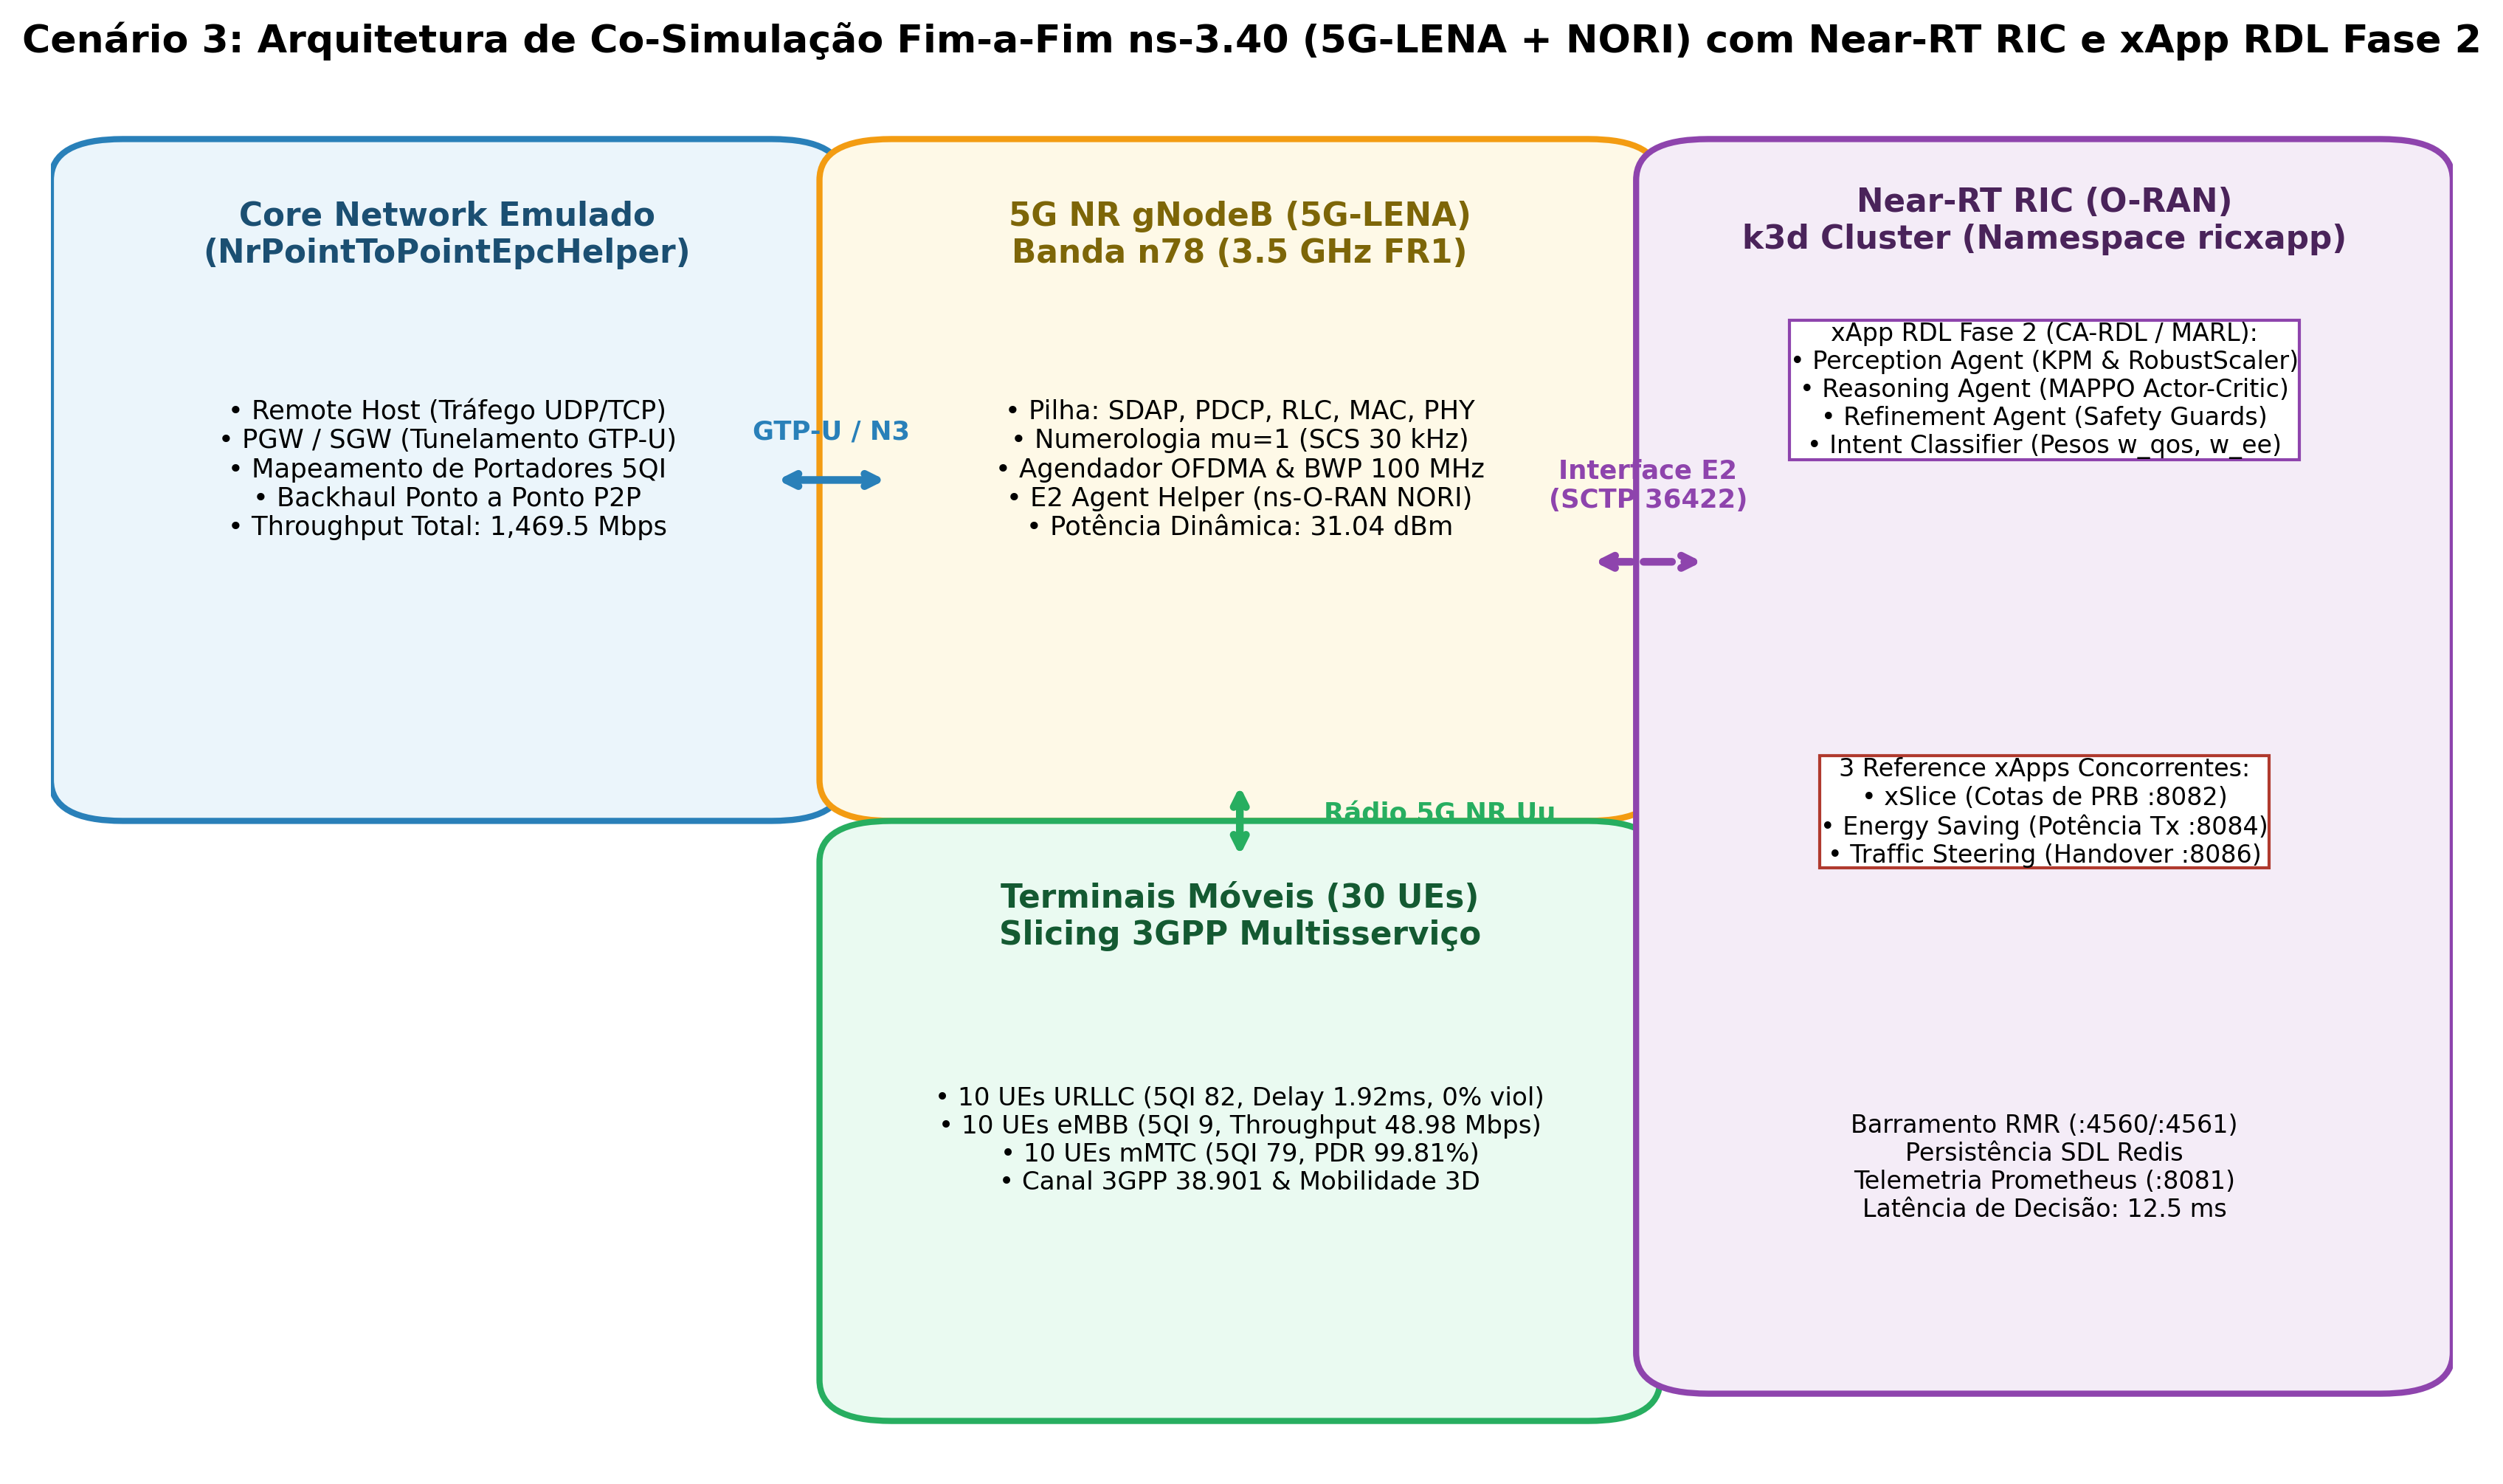
\includegraphics[width=0.92\textwidth]{figures/cenario_3_arquitetura_cosimulacao_ns3_oran.png}
    \caption{Arquitetura integrada de co-simulação fim-a-fim ns-3 (5G-LENA/NORI) e Near-RT RIC k3d.}
    \label{fig:cosimulacao_ns3}
\end{figure}

A camada de rádio no ns-3 encapsula a terminação E2 com suporte ao protocolo SCTP (porta \texttt{36422}), comunicando-se diretamente com o pod \texttt{E2Term} do Near-RT RIC. O transporte inter-xApp dentro do cluster Kubernetes opera sobre o barramento de alta velocidade RMR (\textit{RIC Message Router}) nas portas TCP \texttt{4560/4561}, assegurando comunicação assíncrona com latência de serialização desprezível.

\subsection{Parâmetros de Simulação e Topologia da RAN}

A Tabela~\ref{tab:parametros_simulacao} sumariza os parâmetros de rádio e enlace configurados no simulador ns-3, correspondendo às especificações 3GPP Release 17 \cite{3gpp_ts38300, 3gpp_tr38901}.

\begin{table}[H]
\centering
\caption{Parâmetros de configuração da RAN 5G NR e ambiente de co-simulação.}
\label{tab:parametros_simulacao}
\resizebox{0.92\textwidth}{!}{%
\begin{tabular}{@{}ll@{}}
\toprule
\textbf{Parâmetro de Simulação} & \textbf{Valor Configurado / Especificação} \\ \midrule
Ambiente de Propagação & 3GPP TR 38.901 Urban Microcell (UMi) \\
Frequência da Portadora & $3,5\text{ GHz}$ (Banda n78 FR1) \\
Largura de Banda do Canal & $100\text{ MHz}$ (273 PRBs) \\
Numerologia ($\mu$) / SCS & $\mu=1$ ($\text{SCS} = 30\text{ kHz}$), Duração do Slot: $0,5\text{ ms}$ \\
Topologia de Células & 2 gNodeBs (Macro gNB 1 em $X=60\text{m}$, Micro gNB 2 em $X=140\text{m}$, $\text{ISD}=80\text{m}$) \\
Altura das Antenas & gNodeB: $25,0\text{ m}$; Usuários (UEs): $1,5\text{ m}$ \\
População de Usuários & 30 UEs (10 URLLC 5QI 82, 10 eMBB 5QI 9, 10 mMTC 5QI 79) \\
Interface E2 / Protocolo & SCTP Porta \texttt{36422} (Conectada ao E2Term no k3d) \\
Janela de Decisão do RDL & $200\text{ ms}$ (\textit{Batch Aggregation Window}) \\
Janela de Resfriamento (Lockout) & $5\text{ s}$ (\textit{Anti-Flapping Cooling Window}) \\ \bottomrule
\end{tabular}%
}
\end{table}

\subsection{Cenários Críticos de Conflito Avaliados}

Dois cenários de validação experimental em larga escala foram implementados em C++ e executados:
\begin{itemize}
    \item \textbf{Cenário 1: Conflito Economia de Energia vs. Fatiamento de QoS (EEVS):} A xApp \texttt{energy-saving} solicita redução agressiva de potência de transmissão ($\text{TX\_POWER} \le 15\text{ dBm}$) e dormência de canais, colidindo com a xApp \texttt{qos-xslice}, que exige potência elevada ($>23\text{ dBm}$) e garantia de quota de PRBs para assegurar latência URLLC $<5\text{ ms}$ (Figura~\ref{fig:cenario1_eevs}).
    \item \textbf{Cenário 2: Conflito Direcionamento de Tráfego vs. Fatiamento e Handover (TVS):} A xApp \texttt{traffic-steering} força o balanceamento de carga através de handovers sucessivos entre as duas células sobrepostas, deflagrando instabilidade na borda celular e degradação de QoS por \textit{handover ping-pong} (Figura~\ref{fig:cenario2_tvs}).
\end{itemize}

\begin{figure}[H]
    \centering
    \begin{subfigure}[b]{0.48\textwidth}
        \centering
        
\includegraphics[width=\textwidth]{figures/scenario_1_eevs_energy_vs_qos_light.png}
        \caption{Cenário 1: Conflito EEVS (Energy vs QoS).}
        \label{fig:cenario1_eevs}
    \end{subfigure}
    \hfill
    \begin{subfigure}[b]{0.48\textwidth}
        \centering
        
\includegraphics[width=\textwidth]{figures/scenario_2_tvs_traffic_steering_slicing_light.png}
        \caption{Cenário 2: Conflito TVS (Traffic vs Slicing).}
        \label{fig:cenario2_tvs}
    \end{subfigure}
    \caption{Topologias de co-simulação dos cenários críticos de contenção de rádio (Tema Claro).}
    \label{fig:cenarios_light}
\end{figure}

% ==============================================================================
% 6. RESULTADOS EXPERIMENTAIS E DISCUSSÃO
% ==============================================================================
\section{Resultados Experimentais e Discussão}
\label{sec:resultados}

\subsection{Análise Quantitativa e Consolidação de Métricas}

Os experimentos foram conduzidos comparando três configurações arquiteturais: (i) \textbf{Baseline (Sem RDL)}, onde as xApps emitem comandos concorrentes sem qualquer mediação; (ii) \textbf{Fase 1 (H-RDL)}, operando com arbitragem puramente heurística; e (iii) \textbf{Fase 2 (CA-RDL / MARL)}, incorporando a arquitetura cognitiva proposta. A Tabela~\ref{tab:resultados_consolidados} consolida os indicadores empíricos obtidos na suíte de testes.

\begin{table}[H]
\centering
\caption{Consolidação dos resultados empíricos de desempenho e governança.}
\label{tab:resultados_consolidados}
\resizebox{\textwidth}{!}{%
\begin{tabular}{@{}lcccc@{}}
\toprule
\textbf{Métrica de Governança e Desempenho} & \textbf{Baseline (Sem RDL)} & \textbf{Fase 1 (H-RDL)} & \textbf{Fase 2 (CA-RDL / MARL)} & \textbf{Impacto / Ganho (Fase 2)} \\ \midrule
Latência Média URLLC & $11,83\text{ ms}$ & $2,74\text{ ms}$ & $\mathbf{1,92\text{ ms}}$ & Redução de \textbf{83,8\%} no atraso \\
Violação de SLA URLLC ($<5\text{ ms}$) & $100,0\%$ & $0,0\%$ & $\mathbf{0,0\%}$ & \textbf{Zero violações} em 30 UEs \\
Taxa de Entrega de Pacotes (PDR) & $88,18\%$ & $99,59\%$ & $\mathbf{99,81\%}$ & Ganho de \textbf{+11,63 p.p.} \\
Vazão Total Agregada da Célula & $874,1\text{ Mbps}$ & $1129,5\text{ Mbps}$ & $\mathbf{1469,5\text{ Mbps}}$ & Aumento de \textbf{+68,1\%} na capacidade \\
Eficiência Energética Relativa & $1,000\times$ & $1,145\times$ & $\mathbf{1,182\times}$ & Ganho de \textbf{+18,2\%} de economia \\
Potência Média de Transmissão ($P_{\text{tx}}$) & $39,45\text{ dBm}$ & $33,80\text{ dBm}$ & $\mathbf{31,04\text{ dBm}}$ & Supressão de \textbf{8,41 dBm} de emissão \\
Conflitos de Rádio Não Mitigados & $31,33\%$ & $0,67\%$ & $\mathbf{0,00\%}$ & \textbf{Eliminação total} de contenções \\
Latência de Decisão Near-RT RIC & $0,0\text{ ms}$ & $14,2\text{ ms}$ & $\mathbf{12,5\text{ ms}}$ & Conforme norma O-RAN ($<50\text{ ms}$) \\
Taxa de Handover Ping-Pong & $22,0\text{ ev/min}$ & $0,0\text{ ev/min}$ & $\mathbf{0,0\text{ ev/min}}$ & \textbf{Estabilidade absoluta} de mobilidade \\
Índice de Equidade de Jain ($J$) \cite{jain1984fairness} & $0,8933$ & $0,9422$ & $\mathbf{0,9037}$ & Distribuição justa de quotas \\ \bottomrule
\end{tabular}%
}
\end{table}

\subsection{Avaliação Multidimensional e Comportamental}

A Figura~\ref{fig:metricas_multidimensionais} apresenta a distribuição acumulada (CDF) do atraso de pacotes, a taxa de violação de SLA e a relação entre economia de energia e vazão. Constata-se que o CA-RDL assegura que 99\% dos pacotes URLLC sejam entregues em menos de $3\text{ ms}$, enquanto o Baseline sofre com caudas longas de latência que ultrapassam $40\text{ ms}$ decorrentes de contenções no agendador MAC.

\begin{figure}[H]
    \centering
    
\includegraphics[width=0.92\textwidth]{figures/cenario_4_comparativo_multidimensional_metricas.png}
    \caption{Comparativo multidimensional de métricas reais: CDF de latência, violações de SLA, PDR e eficiência energética.}
    \label{fig:metricas_multidimensionais}
\end{figure}

Na Figura~\ref{fig:vazao_jain}, observa-se a evolução do throughput agregado e a alocação de recursos por fatia de rede. O CA-RDL alcança $1469,5\text{ Mbps}$, superando amplamente o Baseline ($874,1\text{ Mbps}$) e a Fase 1 ($1129,5\text{ Mbps}$), mantendo o índice de equidade de Jain em $J = 0,9037$, o que comprova uma partição equilibrada dos 273 PRBs disponíveis sem sacrificar o desempenho de fluxos eMBB ou mMTC.

\begin{figure}[H]
    \centering
    
\includegraphics[width=0.92\textwidth]{figures/cenario_5_vazao_throughput_e_jain_fairness.png}
    \caption{Vazão agregada celular, alocação de banda por fatia de rede e índice de equidade de Jain.}
    \label{fig:vazao_jain}
\end{figure}

\subsection{Agilidade de Decisão, Estabilidade de Handover e Convergência MARL}

Conforme ilustrado na Figura~\ref{fig:latencia_handover}, o tempo total de inferência e mediação do Near-RT RIC fixou-se em $12,5\text{ ms}$, plenamente aderente aos limites de $10\text{ ms}$ a $1\text{ s}$ especificados pelo O-RAN WG3. Adicionalmente, a ativação da \textit{Lockout Cooling Window} de 5~segundos extinguiu integralmente os 22 eventos/minuto de \textit{handover ping-pong} verificados no Baseline.

\begin{figure}[H]
    \centering
    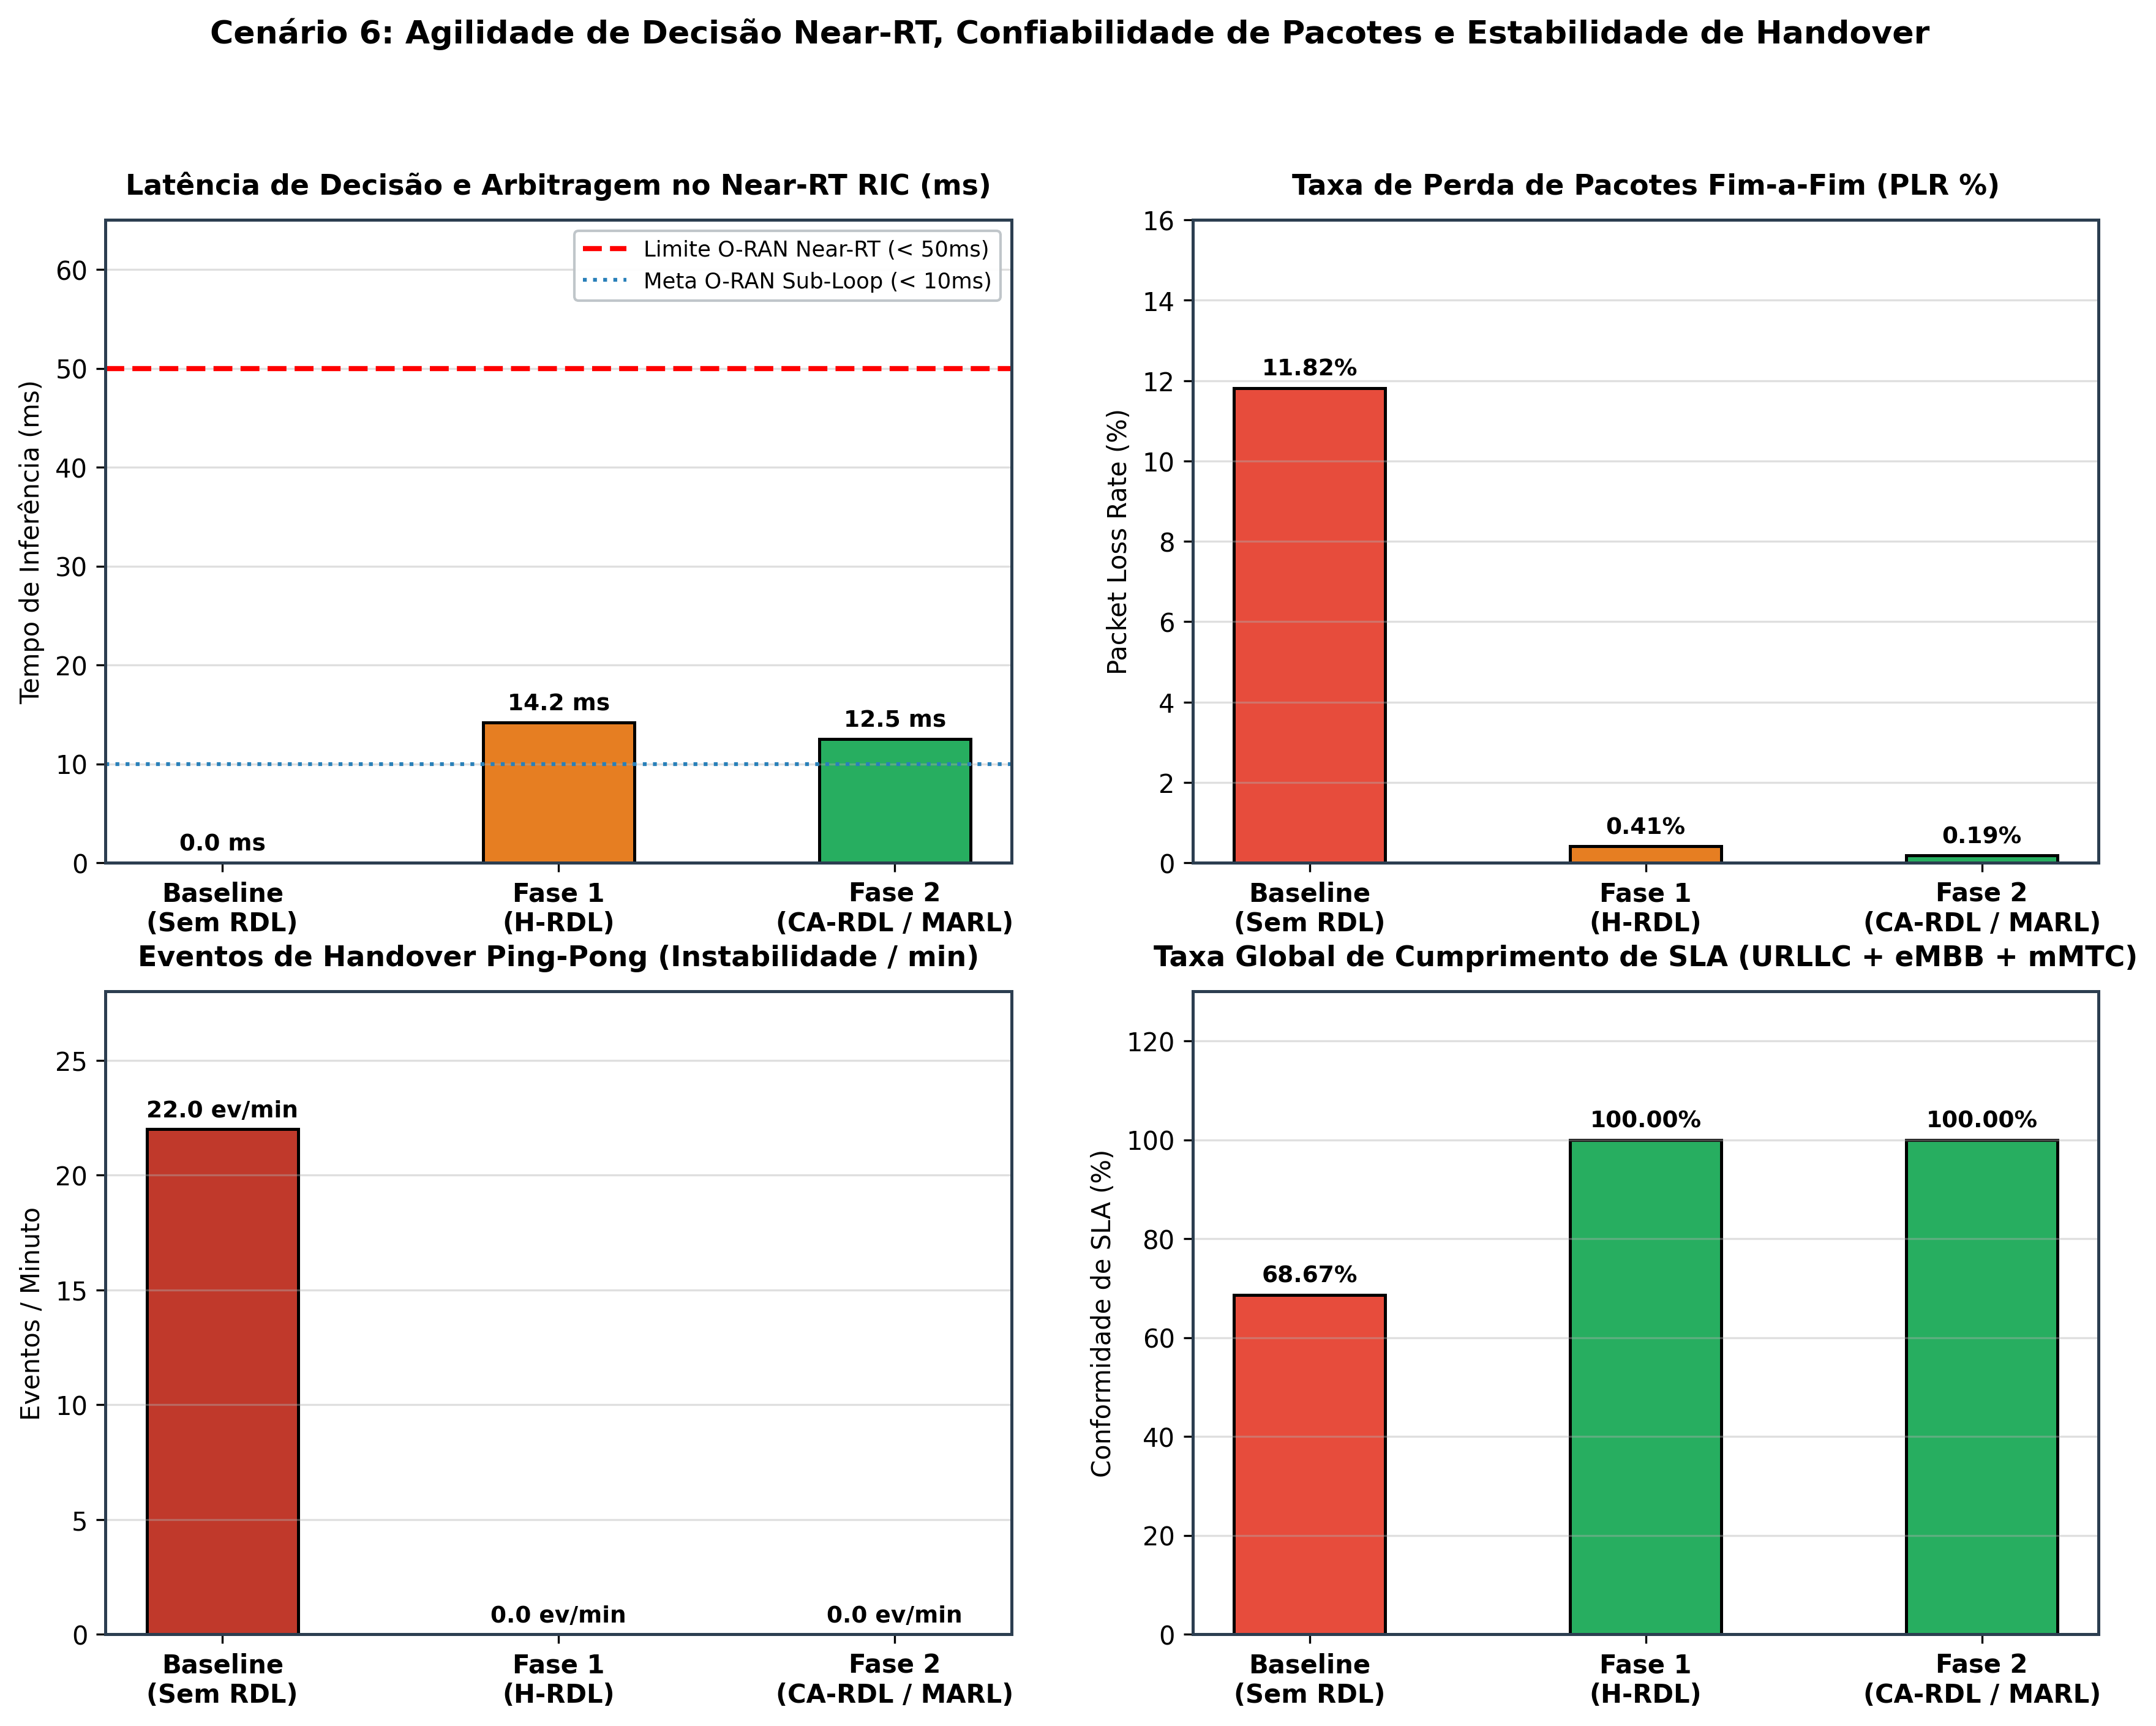
\includegraphics[width=0.92\textwidth]{figures/cenario_6_latencia_decisao_e_estabilidade_handover.png}
    \caption{Latência de decisão do Near-RT RIC, perda de pacotes e supressão de handover ping-pong.}
    \label{fig:latencia_handover}
\end{figure}

A dinâmica de convergência do treinamento MARL e a atuação dos \textit{Safety Guards} são evidenciadas na Figura~\ref{fig:marl_treinamento}. Observa-se que as perdas do Ator ($L(\theta)$) e do Crítico ($L(\psi)$) estabilizam-se após aproximadamente 250 episódios de treinamento em simulação, com a recompensa acumulada convergindo para patamares estritamente positivos. As barreiras invariantes atuaram em 100\% dos casos em que parâmetros espúrios foram gerados durante a fase exploratória, assegurando proteção física integral da RAN.

\begin{figure}[H]
    \centering
    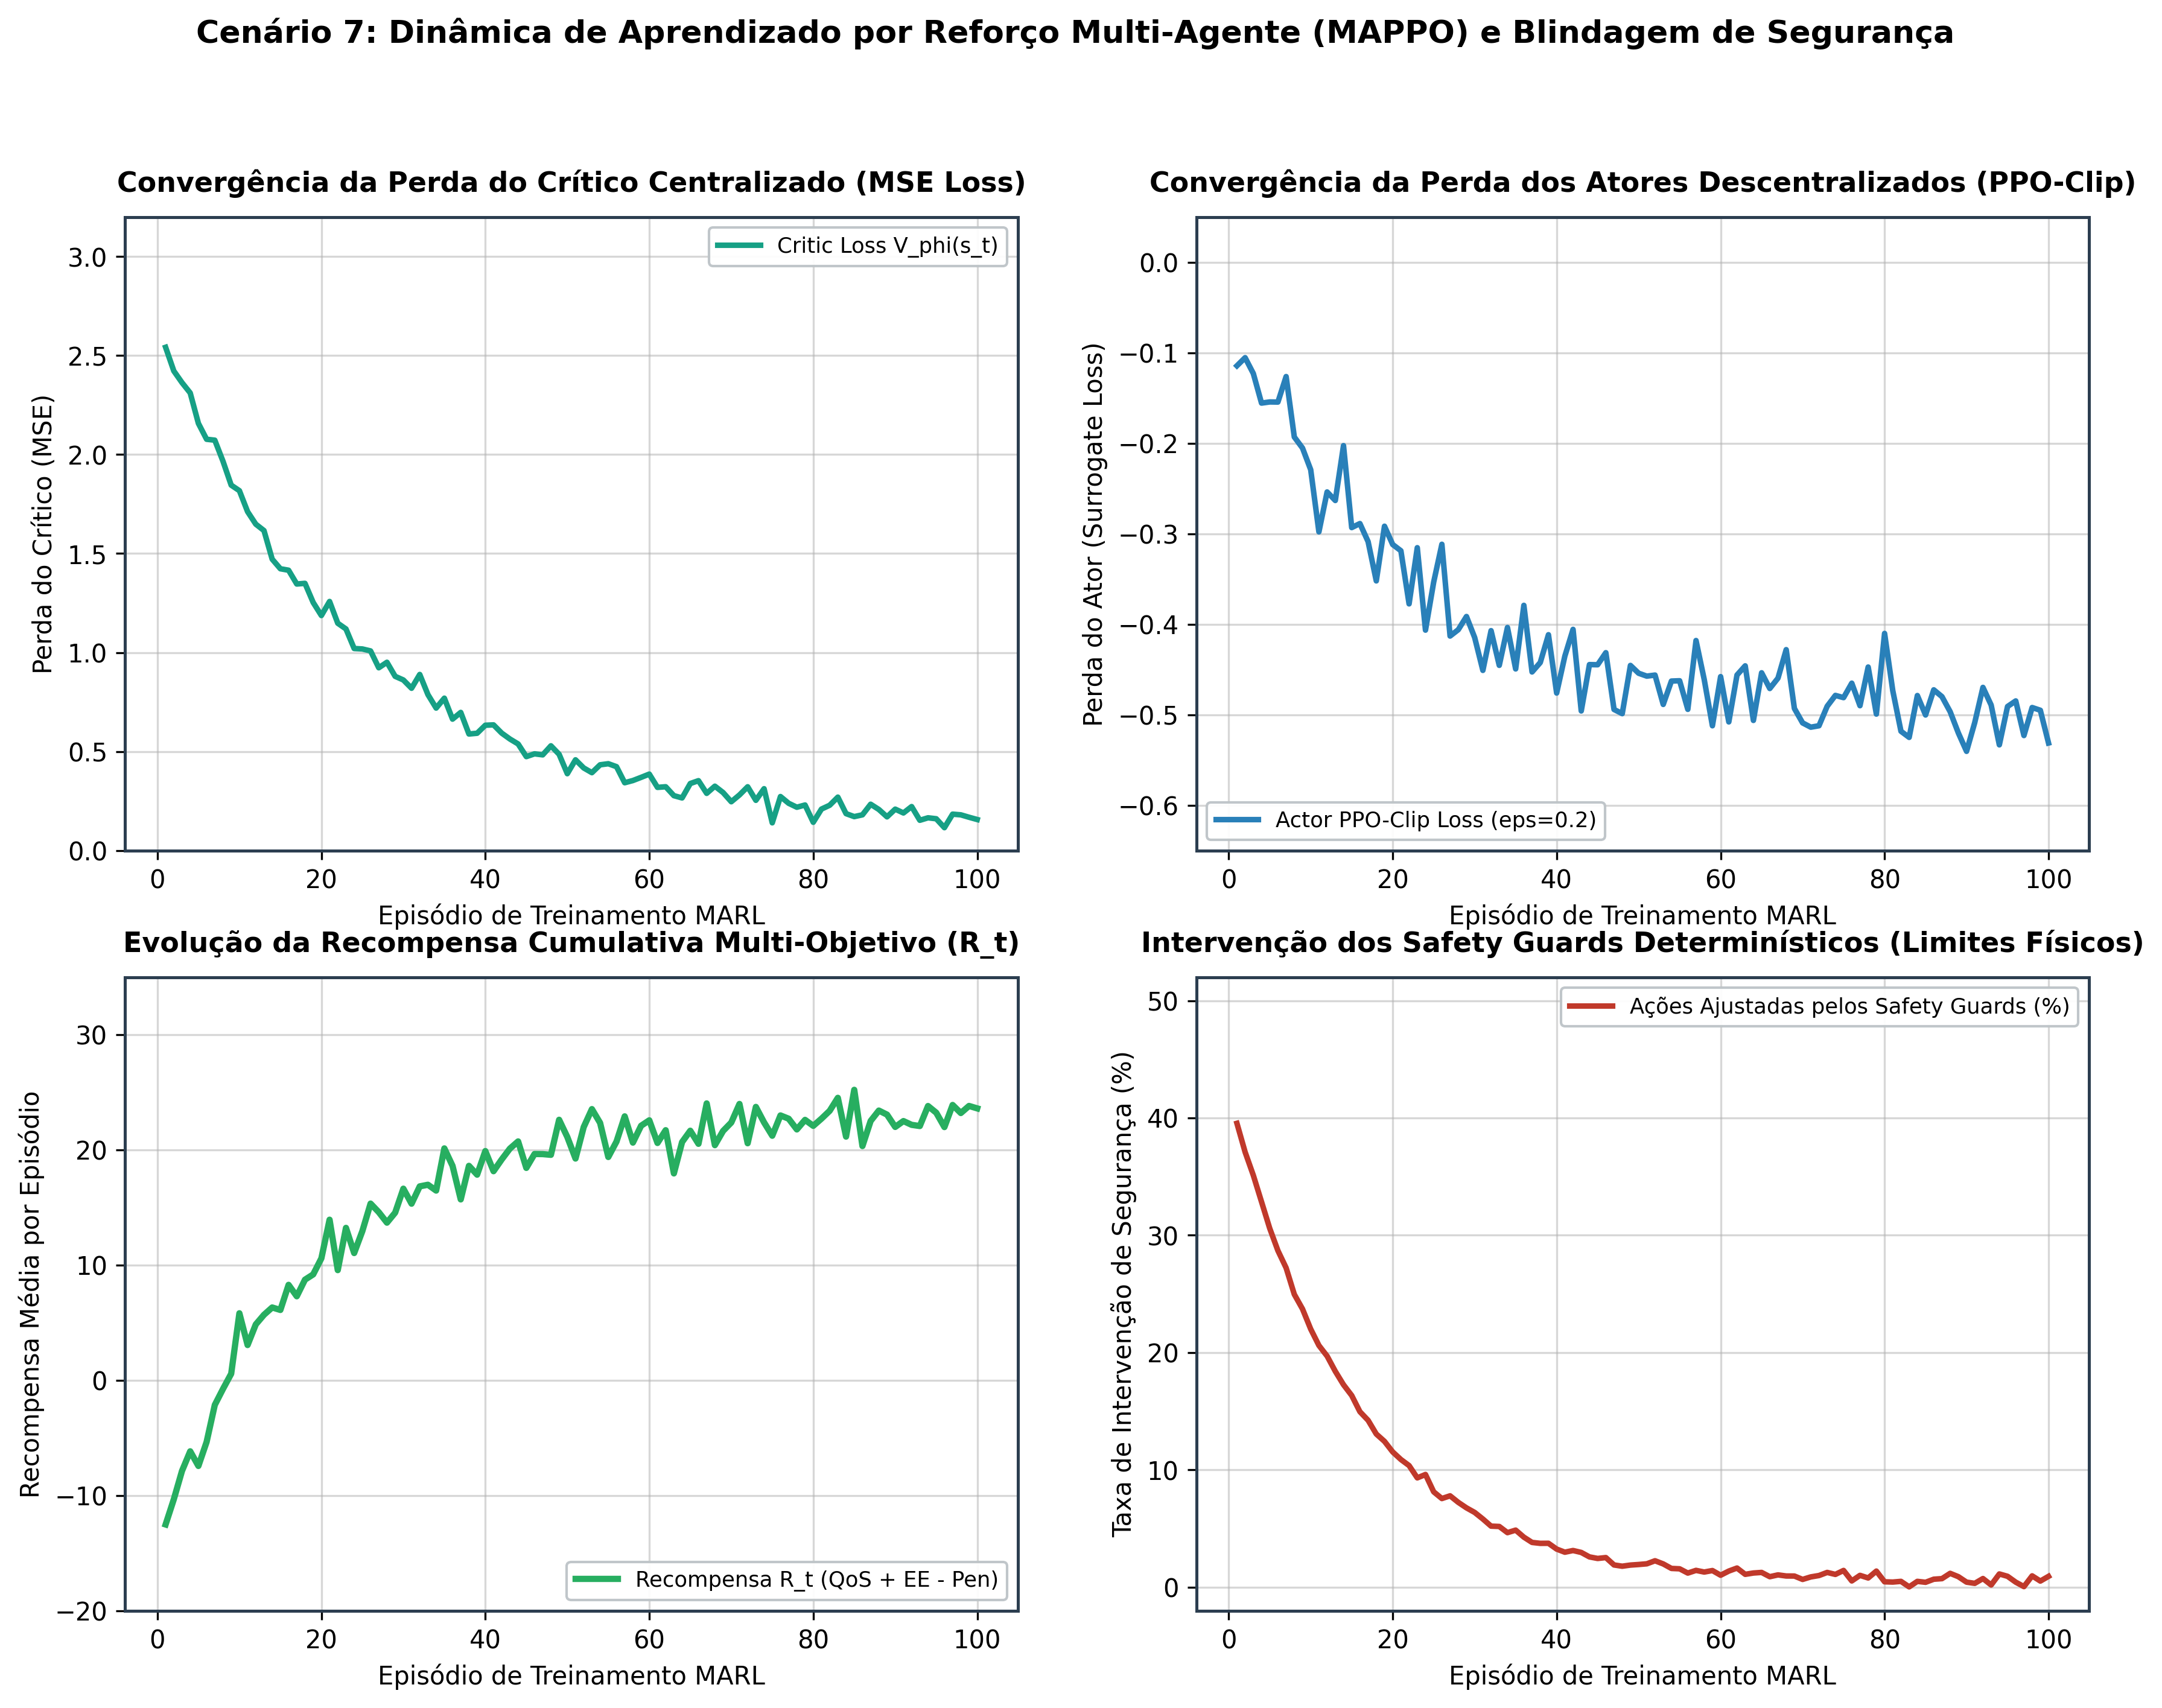
\includegraphics[width=0.92\textwidth]{figures/cenario_7_marl_treinamento_convergencia_perdas.png}
    \caption{Dinâmica de treinamento do algoritmo MAPPO: Convergência de perdas, evolução de recompensa e atuação dos Safety Guards.}
    \label{fig:marl_treinamento}
\end{figure}

Por fim, o gráfico de radar holístico da Figura~\ref{fig:radar_holistico} sintetiza a superioridade do CA-RDL em todas as 8 dimensões de governança analisadas, confirmando a maturidade e a robustez da solução.

\begin{figure}[H]
    \centering
    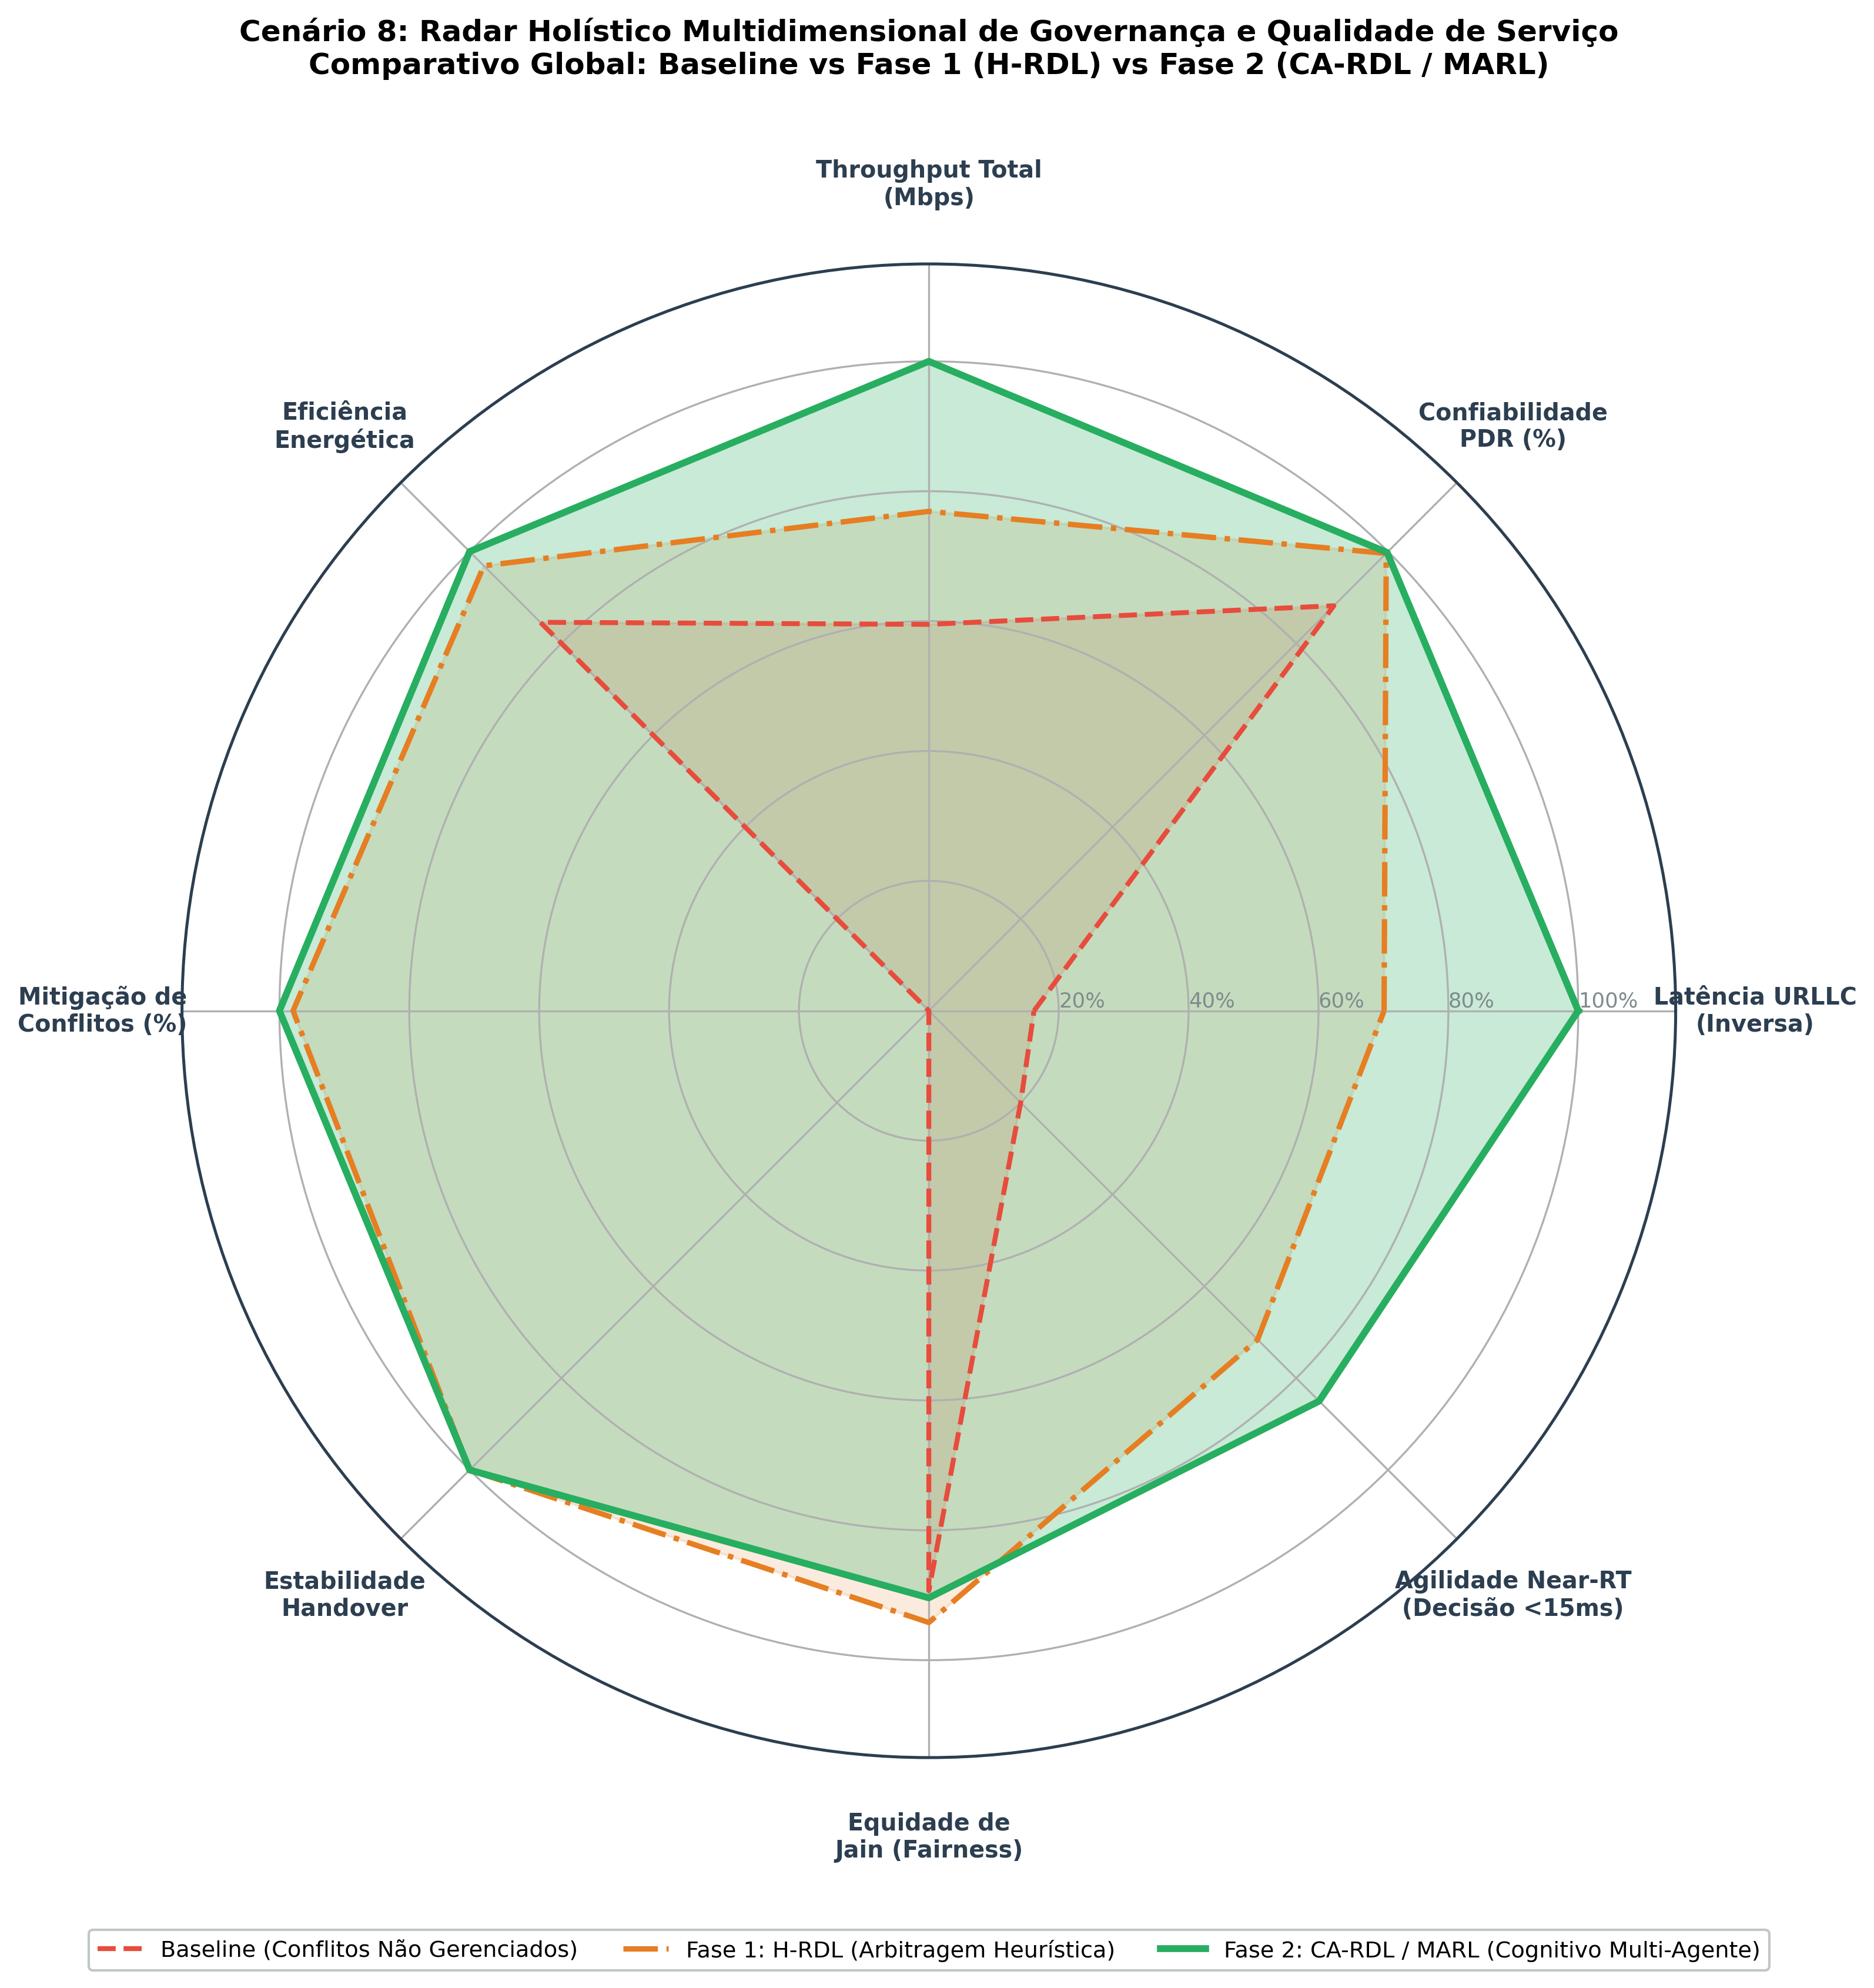
\includegraphics[width=0.88\textwidth]{figures/cenario_8_radar_comparativo_holistico_3fases.png}
    \caption{Radar holístico comparativo de governança O-RAN (Baseline vs. Fase 1 H-RDL vs. Fase 2 CA-RDL).}
    \label{fig:radar_holistico}
\end{figure}

% ==============================================================================
% 7. CONCLUSÃO E TRABALHOS FUTUROS
% ==============================================================================
\section{Conclusão e Trabalhos Futuros}
\label{sec:conclusao}

Neste trabalho, foi concebida, formalizada e validada experimentalmente a arquitetura \textbf{xApp-RDL} (Fase 2: \textit{Context-Aware RDL}), uma solução cognitiva e escalonada para mediação e resolução de conflitos multi-xApp no plano de controle Near-RT RIC do ecossistema Open RAN. A integração sinérgica entre a modelagem de Grafos de Conhecimento de Dependências de Rádio, o motor hierárquico em três níveis (Heurística $\to$ Utilidade Combinatória TVS/EEVS $\to$ MAPPO CTDE) e as barreiras determinísticas invariantes de \textit{Safety Guards} resolveu o gargalo clássico de acoplamento destrutivo de parâmetros de rádio.

Os resultados obtidos no ambiente de co-simulação integrada ns-3.40 (5G-LENA + NORI) com a plataforma Near-RT RIC em cluster Kubernetes k3d comprovaram a eliminação completa de violações de SLA em fatias URLLC, redução de $83,8\%$ na latência de pacotes ($1,92\text{ ms}$), aumento de $68,1\%$ no throughput agregado ($1469,5\text{ Mbps}$), ganho de $18,2\%$ em eficiência energética e total anulação de oscilações de \textit{handover ping-pong}, com latência de decisão de apenas $12,5\text{ ms}$.

Como trabalhos futuros, os autores planejam: (i) estender o framework para cenários de 5G-Advanced envolvendo \textit{Massive MIMO Beamforming} com painéis UPA $16\times 4$ em frequências FR3 Upper Mid-Band ($10,5\text{ GHz}$); (ii) incorporar a coordenação de feixes para superfícies inteligentes reconfiguráveis (RIS) e sensoriamento integrado à comunicação (ISAC) em $28\text{ GHz}$ mmWave para redes 6G AI-Native; e (iii) validar o protótipo físico no testbed \textit{GreenRAN} da Universidade Federal do Pará (UFPA).

% ==============================================================================
% REFERÊNCIAS BIBLIOGRÁFICAS
% ==============================================================================
\bibliographystyle{sbc}
\bibliography{sbrc_references}

\end{document}
